%Pavel Chvykov


% ***********************************************************
% ******************* MY HEADER ************************
% ***********************************************************
\documentclass[11pt]{article}
%\documentclass[prb]{revtex4-1}
%\documentclass[twocolumn,showpacs,preprintnumbers,amsmath,amssymb,superscriptaddress]{revtex4-1}
%\usepackage[greek, english]{babel}

\usepackage{amsmath} % AMS Math Package
\usepackage{amsthm} % Theorem Formatting
\usepackage{amssymb}	% Math symbols such as \mathbb
\usepackage[pdftex]{graphicx}
\usepackage{epstopdf}
\usepackage{enumerate}
%\usepackage{multicol} % Allows for multiple columns
\usepackage{wrapfig}
\usepackage[dvips,letterpaper,margin=1in,bottom=1in]{geometry}
\usepackage{color}
\usepackage{tensind}
\tensordelimiter{`}
\whenindex{a}{\alpha}{} \whenindex{b}{\beta}{} \whenindex{g}{\gamma}{} \whenindex{d}{\delta}{} \whenindex{e}{\varepsilon}{} \whenindex{m}{\mu}{} \whenindex{n}{\nu}{} \whenindex{l}{\lambda}{} \whenindex{k}{\kappa}{} \whenindex{r}{\rho}{} \whenindex{s}{\sigma}{} \whenindex{t}{\tau}{}
\usepackage{todonotes}
\usepackage{subcaption}
% % Sets margins and page size
%\pagestyle{empty} % Removes page numbers
\usepackage{setspace}
%\onehalfspacing
%\setstretch{1.1}
\usepackage{comment}
\usepackage{cancel}
%\usepackage{xfrac}
\usepackage[]{units}

\usepackage{hyperref}
\usepackage[all]{hypcap}
\makeatletter % Need for anything that contains an @ command 

%\renewcommand{\maketitle} % Redefine maketitle to conserve space
%{ \begingroup \vskip 10pt \begin{center} \Large {\bf \@title}
%		\vskip 10pt \large \@author \\ \@date \end{center}
%		\vskip 10pt \endgroup \setcounter{footnote}{0} }


%\makeatother % End of region containing @ commands
%\renewcommand{\labelenumi}{(\alph{enumi})} % Use letters for enumerate
% \DeclareMathOperator{\Sample}{Sample}
\let\vaccent=\v % rename builtin command \v{} to \vaccent{}
\renewcommand{\v}[1]{\ensuremath{\vec{#1}}} % for vectors
\newcommand{\gv}[1]{\ensuremath{\mbox{\boldmath$ #1 $}}} 
% for vectors of Greek letters
\newcommand{\uv}[1]{\ensuremath{\mathbf{\hat{#1}}}} % for unit vector
\newcommand{\abs}[1]{\left| #1 \right|} % for absolute value
\newcommand{\avg}[1]{\left< #1 \right>} % for average
\let\underdot=\d % rename builtin command \d{} to \underdot{}
\renewcommand{\d}[2]{\frac{d #1}{d #2}} % for derivatives
\newcommand{\dd}[2]{\frac{d^2 #1}{d #2^2}} % for double derivatives
\newcommand{\pd}[2]{\frac{\partial #1}{\partial #2}} 
% for partial derivatives
\newcommand{\pdd}[2]{\frac{\partial^2 #1}{\partial #2^2}} 
% for double partial derivatives
\newcommand{\pdc}[3]{\left( \frac{\partial #1}{\partial #2}
\right)_{#3}} % for thermodynamic partial derivatives
\newcommand{\fd}[2]{\frac{\delta #1}{\delta #2}} %functional derivative
\newcommand{\fdd}[3]{\frac{\delta^2 #1}{\delta #2 \delta #3}} %second functional derivative
\newcommand{\ket}[1]{\left| #1 \right>} % for Dirac bras
\newcommand{\bra}[1]{\left< #1 \right|} % for Dirac kets
\newcommand{\braket}[2]{\left< #1 \vphantom{#2} \right|
\left. #2 \vphantom{#1} \right>} % for Dirac brackets
\newcommand{\matrixel}[3]{\left< #1 \vphantom{#2#3} \right|
#2 \left| #3 \vphantom{#1#2} \right>} % for Dirac matrix elements
\newcommand{\grad}{\nabla} % for gradient
\let\divsymb=\div % rename builtin command \div to \divsymb
\renewcommand{\div}[1]{\gv{\nabla} \cdot #1} % for divergence
\newcommand{\curl}[1]{\gv{\nabla} \times #1} % for curl
\newcommand{\tr}{\mbox{Tr}}
\let\baraccent=\= % rename builtin command \= to \baraccent
\renewcommand{\=}[1]{\stackrel{#1}{=}} % for putting numbers above =
\renewcommand{\deg}{^{\circ}} %degree simbol
\renewcommand{\(}{\left (}
\renewcommand{\)}{\right  )}
\renewcommand{\[}{\left [}
\renewcommand{\]}{\right ]}
\newcommand{\<}{\left <}
\renewcommand{\>}{\right >}

\newtheorem{prop}{Proposition}
\newtheorem{thm}{Theorem}[section]
\newtheorem{lem}[thm]{Lemma}
\theoremstyle{definition}
\newtheorem{dfn}{Definition}
\theoremstyle{remark}
\newtheorem*{rmk}{Remark}
\newtheorem{?}{\textbf{Question}}

\newcommand{\e}[1]{\mbox{e}^{#1}} %exponential
\renewcommand{\exp}[1]{\mbox{exp}\[#1\]} %exponential
\newcommand{\intmom}[2][4]{\int \frac{d^{#1} #2}{(2\pi)^{#1}}} % 4D momentum integral
\newcommand{\intfn}{\int \mathcal{D}} %functional integral
\newcommand{\D}{\mathcal{D}}
\newcommand{\bigO}[1]{O(#1)}  %order of (big O notation)
\newcommand{\Op}{\mathcal{O}}  %operator
\newcommand{\im}{i}  %imaginary
\renewcommand{\todo}[1]{\textit{\color{red}[#1]}}
\newcommand{\um}{$ \mathrm{\mu} $m}
\renewcommand{\inf}{\infty}
\newcommand{\with}{\quad \text{with} \quad}
% ***********************************************************
% ********************** END HEADER *************************
% ***********************************************************

\begin{document}
		\title{Least Rattling in Smarticles}
		
		\author{author list} %\thanks{pchvykov@mit.edu}
		
		\maketitle


\tableofcontents

\begin{itemize}
	\item Introduction
	\item regularization in smarticles
	\item Effective noise Teff, correlation
	\item Other configurations: random, phase-offset
	\item breaking this - inertial (do exp't with less inertia?)
	\item RWRM -- graph and diffusion
	\subitem as max-caliber
	\item Discussion
\end{itemize}

\section{Introduction}

\section{Smarticles}
We conducted our experiments with a collection of small simple robots called ``Smarticles'' (smart active particles) (fig. \ref{fig:smarticle}). Each one is comprised of three connected links, with the two hinges being controlled by a programmable micro-controller via stepper motors. When the Smarticle is sitting on its base, the arms do not touch the ground, and so an individual smarticle cannot move. A group of them, on the other hand, can achieve complex motion by pushing off each other. Here we will focus on the regime where their arms are executing a periodic motion pattern, which we call ``gait,'' with no feedback from the environment (note that the gait timing is kept by the controller, and hence the cycle's phase is not affected by forces on the arms). Such gaits can be represented (uniquely up to rate) as closed loops in the two-dimensional conformation space (the two hinge angles) of the Smarticle (fig. \ref{fig:smarticle}). In the first part of the paper, we will have all Smarticles execute a synchronized ``square'' gait (fig. \ref{fig:smarticle}). \todo{Include all the technical details of realization and construction of Smarticles and synchronization in an appendix?}


\begin{figure} 
	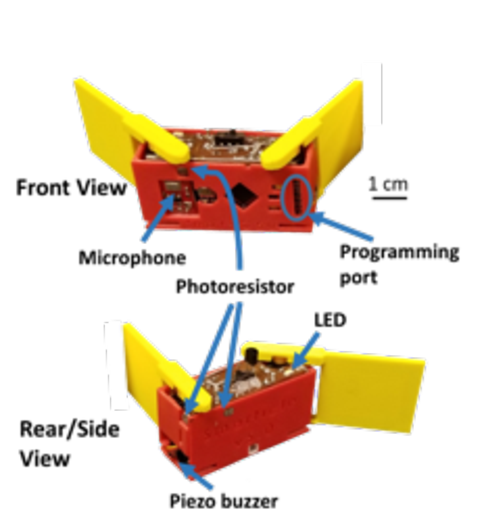
\includegraphics[width=0.3\textwidth]{Smarticle.pdf}
	\caption{\todo{label base} single smarticle with various sensors labelled}
	\label{fig:smarticle}
\end{figure}

We place three Smarticles on a flat aluminium plate, inside a glued-down plastic ring (fig. \ref{fig:super3}). By moving their arms, the robots can push off each other, while the ring prevents them from decoupling -- thus forming an optimal play-ground to look for dynamical emergence. To get data, we use Optitrack \todo{details} to track the full time-evolution of the 2D coordinates and body-angle $ (x,y,\theta) $ of each robot at 120 frames per second (we do not track the arm positions). 

For experiment prototyping and better sampling statistics, we have also built a simulation of this setup, described in Appendix \ref{app:simulation}, and benchmarked it against experiments. Both experimental and simulation data are then fed through a pre-processing pipe-line, which mods out the rotation and permutation symmetries of the 3-Smarticle setup, thus reducing the effective configuration space substantially (Appendix \ref{app:dataAnal}).

\begin{figure}
	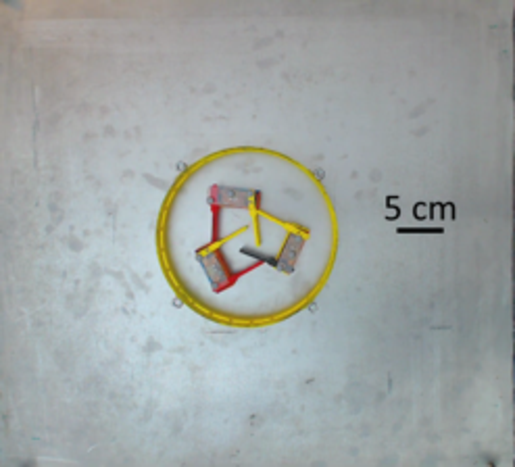
\includegraphics[width=0.3\textwidth]{3smRg.pdf}
	\caption{View from above. Regular state testing setup. The whole setup placed on an aluminum plate leveled to $ < 0.1\deg $. The ring is 19.2 cm in diameter, and is glued to the plate below such that it cannot move or deform. The smarticles perform a square gait locked in phase with each other.}
	\label{fig:super3}
\end{figure}

\section{Regularization}
When all the Smarticles are executing a phase-synchronized square gait, the triplet typically organizes into one of several periodic dynamical patterns (a sort of collective organized dance) \todo{videos in supplement}. Figure \ref{fig:configSpace} gives some illustration of the fine-tuning associated with this \todo{better visualization of regular states???}. Such self-organization is perplexing, and its interpretation depends on the perspective we take -- that of dynamical systems theory, or thermodynamics.
\todo{not synchronization}

\begin{figure}
	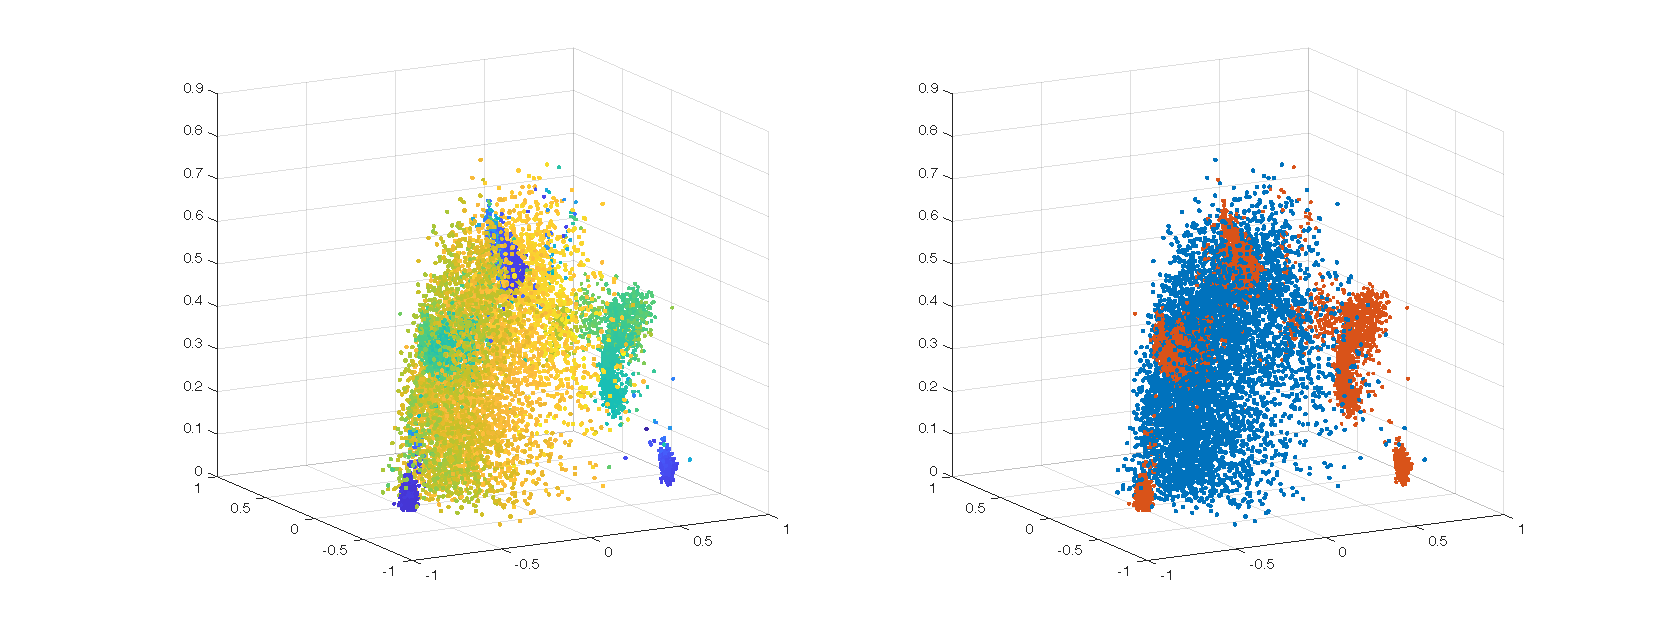
\includegraphics[width=0.7\textwidth]{scatter_FT.pdf}
	\caption{Stroboscopic, 3D projection resolving clusters, of some function of the 9D space (see \ref{app:dataAnal}), ordered v null, color by delta over one period \todo{use exp't data for ordered, and simulation for null}
	\todo{regular states for different drives on same axes}}
	\label{fig:configSpace}
\end{figure}

From the context of dynamical systems, perhaps it is not surprising that the dynamics of a time-periodic system are governed by several limit-cycle attractors. On the other hand, not all periodic systems relax to such attractors -- even here we can make slight changes to our setup, such as changing relative gait phases, or making Smarticles inertial \todo{figures for this here?}, so as to make the system behave chaotically. Furthermore, this system cannot really be seen as deterministic, as we know that it is strongly affected by the stochasticity coming from the hard-boundary interactions between non-smooth shapes, and highly surface-sensitive effects of sliding friction.

From the perspective of equilibrium thermodynamics, where entropy and disorder tend to a maximum, this sort of self-organization may seem extremely surprising. Of course, this system is far from equilibrium, and so entropy need not grow. Indeed, for a Brownian particle diffusing in a compact domain of inhomogeneous temperature $ T(\v{x}) $ (and no other forces), we know that the steady-state probability distribution will be $ p_{s.s.} \propto 1/T(\v{x}) $ -- which can be far from the maximum-entropy uniform distribution. We want to use this example to motivate our explanation of the fine-tuning we observe.

Indeed, the intuition is the same: probability concentrates in regular states, which are, in some sense, less noisy than the chaotic behavior in other parts of the configuration space. We can make this intuition precise by defining an effective temperature $ T_{eff}(\v{x}) $ at every point in the configuration space, and checking if it correlates with $ p_{s.s.}(\v{x}) $. While this system is too complicated to calculate $ T_{eff} (\v{x})$ from first principles, we can ``measure'' it numerically from ensembles of short trajectories starting at $ \v{x} $. Our hypothesis, therefore, is that we can predict the long-term behavior from looking only at short trajectories -- which need not be possible for far-from-equilibrium systems. 

%While we could try to go into a mechanistic explanation for the self-organization in our setup, it would likely be very specific to the parameters and choices used here and would not generalize well to other configurations of Smarticles, or to other active matter systems. Instead, we want to give a less fundamental, but more generalizable explanation. We note that for most initial configurations of the three Smarticles in a ring, after one period of arm motion they go to a new configuration. For some specific configurations, however, they stay in the same place -- and these are precisely the periodic limit-cycle attractors we see in any long trajectory (fig. \ref{fig:configSpace}). This may at first seem tautological: at long times the system tends to be found in places from where it does not leave. The rest of the paper will be explaining why this is both, highly non-trivial in a precise mathematical sense, and also profound for understanding real-world strongly-driven systems \todo{references to sections}.

\section{Defining $ T_{eff} $}
The question, therefore, is how can we extract a measure of effective noise amplitude from looking at short trajectories. On one hand this system is periodic in time, so one natural metric would be to look at the distance it moves in configuration space over one period. Another natural metric could be inspired by Brownian dynamics $ \dot{x}=\sqrt{2\;T(x)}\cdot\xi $, and so $ T(x)=\int dt\;\<\dot{x}(t)\;\dot{x}(0)\>/2 $, or in higher dimension, we can take the trace of the correlator $ T(x)=\sum_i\<\dot{x}_i\;\dot{x}_i\>/2 $. 
We then color the points in fig. \ref{fig:configSpace} by this $ T_{eff} $, and see that the regions of low $ T_{eff} $ correspond precisely to the concentration of steady-state probability. More precisely, fig. \todo{fig:corr} shows the scatter plot of $ p_{s.s.}(x) $ vs. $ T_{eff}(x) $, showing the correlation.

Note that this may at first seem tautological: at long times the system tends to be found in places from where it does not leave. However, below we will explain why this is both, highly non-trivial in a precise mathematical sense, and also profound for understanding real-world strongly-driven systems 

\section{Drive-specificity}
Why should a driven dynamical system get an inhomogeneous $ T_{eff}(x) $ landscape? For a given form of the drive signal, different system configurations will have a different response. In particular, some configurations will respond in a more predictable way than others. In our Smarticle setup, for some initial conditions the sources of stochasticity (such as corner collisions) will be more prevalent than elsewhere. This way, a system settles into drive-specific configurations that give more orderly and stable response properties, and changing the drive will change these selected states. For Smarticles, this would imply that the regular states found at long times are specific to the gait, which is confirmed in experiments (fig. \todo{different gait reg states}). To illustrate that our approach generalizes beyond periodically-driven systems, we can even make the gait random in time, though identical across Smarticles to allow diversity of response properties \todo{figure}.

Another prediction we can make from our framework is that raising the apparent noise uniformly for all configurations $ T_{eff}(\v{x}) \rightarrow T_{eff}(\v{x})+T_0$ will effectively level the steady-state distribution for a large enough $ T_0 $, and thus break the regularization we observe. Experimentally we can realize this by putting smarticles on top of a bed of small, light beads (fig. \todo{smarticles on beads}), thus effectively reducing the friction between Smarticles and the table. This makes every interaction have a larger and less predictable effect, which affects all states in a very similar manner.

%This results in certain configurations being selected by any given drive as having a lower effective noise, and thus becoming attractive. We can illustrate this intuition by changing the gait in our Smarticle system, and seeing new configurations becoming attractive. 


\section{Broader impact}
Our $ T_{eff}(\v{x}) $ is effectively a measure of instability of the configuration $ \v{x} $. Hence, a statement that at steady-state the systems tends to be found in configurations that are more stable (in places it does not leave) may seem tautological at first. However, the key here is that this measure is local -- depends only on the state $ \v{x} $ itself, and not on the rest of the landscape. Landauer's ``blowtorch theorem,'' \todo{cite} on the other hand, shows that for general nonequilibrium systems, the value of the steady-state probability at a point $ \v{x} $ can depend on system properties at any arbitrarily far-away points. Hence having any local quantity that is predictive of the $ p_{s.s.} $ is highly non-trivial and is indicative of additional structure in the system. It can, in some sense, be seen as a generalization of equilibrium thermodynamics -- there, detailed balance ensures that the steady-state is determined locally. In our case, on the other hand, we try to leverage the additional assumption of ``complexity'': we think of our system as so complex, high-dimensional, and ``generic'' that it can essentially be approximated as random. We argue that this is really the ``typical'' scenario -- while it can be violated, such a violation would require fine-tuning, which becomes progressively less likely in more complex high-dimensional systems.

\begin{figure}
	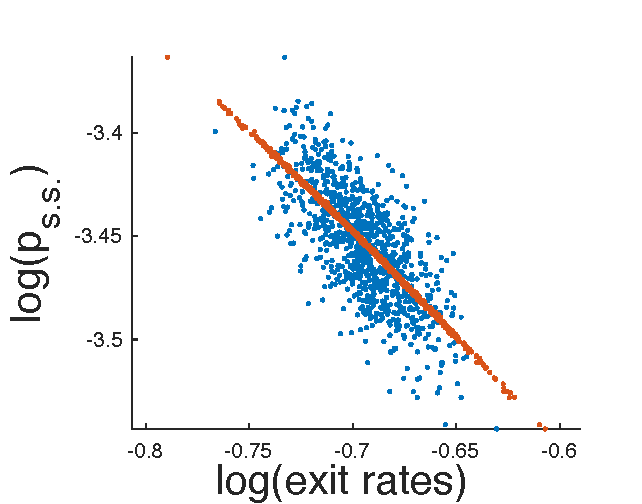
\includegraphics[width=0.55\textwidth]{randMark.pdf}
	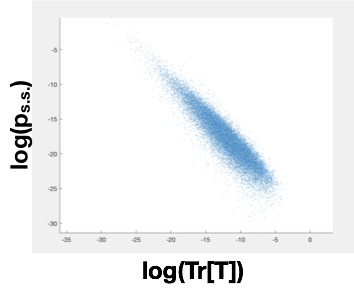
\includegraphics[width=0.45\textwidth]{randDiff.png}
	\caption{a. Steady state for a Markov process with $ 1000 \times 1000 $ random transition matrix. Blue points show exit rates, red points also include the correction from entrance rates.
		%Blue points show $ \frac{\bar{R}}{\sum_j R_{ij}} $, which depends only on the exit rates, and red points also include the correction due to the entrance rates $ +\frac{\sigma}{\bar{R}\,N^{3/2}}\, \xi_i $ 
	b. Steady state vs. trace of temperature tensor for multivariate inhomogeneous diffusion in a random temperature landscape}
	\label{fig:randDynamics}
\end{figure}

There are several ways to make this discussion more precise. One way to look at it is to consider a Markov process $ \dot{p}_i= \sum_j R_{ji}\, p_j - \sum_j R_{ij}\, p_i $, with $ N $ states $ i\in\{1,...,N\} $. In general the steady-state distribution $ p_{s.s.}(i) $ will depend on all the $ N^2 $ transition rates. Now, if we let the transition rates $ R_{ij} $ to be independent identically distributed random variables (with some mean $ \bar{R} $ and standard deviation $ \sigma $), and let $ N \rightarrow \infty$, then it is easy to show \todo{Appx or citation} that $ p_{s.s.}(i)= \frac{1}{N} + \sum_j (R_{ji} - R_{ij})/(N^2\,\bar{R}) + \bigO{N^{-3}}$. The first term $ \sum_j R_{ji} $ is the total entrance rate into state $ i $, and may in a real system be hard to measure, as it would require initializing the system in all possible configurations and seeing how often it enters $ i $. The second term $ \sum_j R_{ij} $, on the other hand, is the total exit rate, and is akin to our measure of $ T_{eff} $ -- it is basically a measure of how stable the state $ i $ is and only requires local measurements initialized in that state. We can rewrite the expression for the steady-state focusing on the exit rates: $ p_{s.s.}(i)= \frac{\bar{R}}{\sum_j R_{ij}} + \frac{\sigma}{\bar{R}\,N^{3/2}}\, \xi_i$, where $ \xi_i \equiv  \sum_j \(R_{ji}-\bar{R}\)/\(\sigma\,\sqrt{N}\)\sim 
\mathcal{N}[0,1]$ -- univariate Gaussian random variable. So while in general we need all $ N^2 $ rates to predict the steady-state, the randomness in rates allows us to express it in terms of just $ N $ local measurements of the exit rates, up to a noise term from  the unobserved entrance rates \ref{fig:randDynamics}a.
%This simple model thus qualitatively reproduces what we observe in the Smarticle system: that exit rate is predictive of the steady-state density, albeit not perfectly because of the additional influence of the entrance rates 

It turns out we can make an even stronger statement if we consider the $ d $-dimensional diffusion process on a compact domain $ \dot{x}_i = D_{ij}(x)\cdot\xi_j $ [Ito], $ i\in\{1,...,d\} $, $ \v{x}\in\mathbb{D}^d $, where the diffusion tensor $ D_{ij} $ varies smoothly over $ x $, but is otherwise random. Again, as this is a non-equilibrium process, in general the steady-state density at any point will depend globally on the diffusion tensor everywhere: $ p_{s.s.}(x) = f_x\[D_{ij}(y)\; |\; y\in \mathbb{D}^d \]$. However, the random choice of $ D_{ij}(x) $ simplifies this result: we can numerically show that $ p_{s.s.}(x) \sim 1/\tr\(T(x)\) $ for $ T \equiv D\, D^T$ \ref{fig:randDynamics}b, as long as the variation of $ \tr\(T(x)\) $ is sufficiently large. 

Finally, we can also frame our results in a somewhat different light. We think of approximating the system behavior by ``typical'' dynamics that match the local fluctuation amplitude of the system $ T_{eff}(x) $. Concretely, we find the maximum-entropy (or ``max-caliber'' \todo{cite}) probability distribution over trajectories $ P[\v{x}(t)] $, constraining the local velocity fluctuations: maximize $ \mathcal{S} = P[x] \;\log\(P[x]\) + \lambda_0 \( \int \mathcal{D} x \;P[x] - 1\) + \int dX \; \lambda(X) \(\sum _i \< \dot{x}_i\,\dot{x}_i\> _X - T_{eff}(X)\)$, where $ \< \dot{x}_i\, \dot{x}_i\> _X \equiv \int \mathcal{D}x \; P[x] \,\int dt \; \dot{x}_i(t) \dot{x}_i(t) \,\delta(x(t) - X) $. This gives $ P[x(t)] \propto \exp{-\sum_i \int dt \; \lambda(x(t))\,\dot{x}_i(t)\dot{x}_i(t)} $, which corresponds to the stochastic process $ \dot{x}_i = \sqrt{2\,T_{eff}(x)}\cdot \xi_i$, whose steady-state distribution is $ p_{s.s.}(x)\propto 1/T_{eff}(x) $. Thus, while the exact dynamics generally give a complicated $ p_{s.s.}(x) $, we can view $1/T_{eff}(x) $ as the least-informative approximation based on only local information.

\todo{coordinate dependence}

%In a sense, we found here a local observable that is predictive of the steady-state density in a complex far-from-equilibrium system. This is surprising -- indeed, Landauer showed \todo{cite blowtorch} that for general nonequilibrium systems, the value of the steady-state probability at a point $ \v{x} $ can depend on system properties at any arbitrarily far-away points -- and hence no local observable can exist that predicts $ p_{s.s.}(\v{x}) $. With additional assumptions however, this can become possible -- e.g., the assumption of detailed balance gives the Boltzmann distribution, which depends only on the local energy (up to normalization). Here, we try to leverage the additional assumption of ``complexity'' -- we think of our system as so complex, high-dimensional, and ``generic'' that it can essentially be approximated as random.








\appendix
\renewcommand{\thesection}{\Alph{section}} 
\section{Experiment details}
Talk about Smarticle synchronization issue and experimental design decisions.

\section{Simulation details} \label{app:simulation}
For easier exploration of hypothesis space of this system, we have constructed a numerical simulation with the following algorithm. We approximate smarticles by three-segment lines (insets in fig. \ref{fig:dimRedSim}). At each time-step, the algorithm moves the arms slightly according to the chosen gait, and then iteratively cycles through smarticle pairs in random order, checking for collisions, and moving one in each pair slightly according to the net interaction force. If there are multiple points of contact for a given pair, the move is a translation in the direction of the total force, otherwise, it is a rotation about a pivot point chosen so as to balance the forces and torques. Choosing which in the pair moves is random, weighted by their relative friction coefficients (as motivated by difficulty of predicting static friction). Note that since a move can create new collisions with other smarticles, it is important to take small steps and iterate. The algorithm continues looping through pairs until all collisions are resolved, then proceeding to the next time-step. While this describes the core of the algorithm, there are a number of bells and whistles necessary to improve its stability and reliability:
\begin{itemize}
	\item  If two arms are near-parallel when they approach each other, they can pass through each other between ticks without ever intersecting. To prevent this, along with collision detection, we must explicitly test for this in each pair. We then store the order of the arms for a few ticks into the future to prevent them passing through each other in any of those times.
	\item In case a smarticle with small friction gets trapped between two others, it might rattle back and forth on each iteration of collision-resolution, with no net effect. To prevent this, we temporarily (until next tick) increase its friction each time a smarticle moves.
	\item In experiment, when resolving collision is too hard, the motor simply does not move (jams up). To allow for that possibility in simulation, we add an exit condition from the collision-resolving loop for when any one smarticle's temporary friction (from last bullet) becomes very large - as this serves as a proxy for how much force a motor must provide. We then move the most colliding arm back to its last time-step, and try collision-resolving again. If everything resolves, that arm will then have a chance to catch up to where it needed to be over the following ticks (its speed being capped at some $ \omega_{max} $).
	\item The resulting simulation turns out to be too clean, despite the multiple stochastic elements of the algorithm, and so dynamical phases much more stable than in experiments. Since we want to study transition statistics, we must find ways to destabilize them. There are a number of places we can add more noise: slight fluctuations of smarticles' positions and angles at each tick, or proportional to each move, randomly varying gait amplitude, varying arm velocity, etc.
	\item The ring boundary is implemented similar to other smarticles, and collisions with it are resolved in the same loop. Alternatively, we can implement weakly confining potential to keep smarticles together in a more smooth way (for different experiments).
\end{itemize}

Even with all these additions, many differences remain between simulation and experiment: smarticles have non-zero thickness in experiments, friction forces between smarticles are often important on collisions, there are relief features on smarticle body not present in simulation that can get caught, etc. The consequence in this system is that while qualitative features can be recovered in the simulation, we don't generally expect quantitative agreement. We guess that these differences may become less important for ensembles with more smarticles -- as universal collective properties start to dominate. We also guess that analytical predictive power of least-rattling, or other similar techniques, could be more applicable in that regime.

\section{Data analysis} \label{app:dataAnal}

Once we have the tracked coordinates of the smarticles, we want to map the data into a ``collective behavior space'' -- something that can usefully inform us about the dynamical patterns of motion, especially those relevant for slow time-scales. This behavior space will typically be very high-dimensional, and to work with it we try to either cluster the data into different discrete behaviors (or dynamical phases), or perform a dimensionality-reduction to embed the data in a 2 or 3 dimensional space we can visualize (and could subsequently cluster if desired). In either case, what we care about is not the location of points in behavior space (which would be arbitrary anyway), but only about the distances between them -- i.e., some measures of similarity of different behaviors. 

The raw data from particle tracking gives position and orientation time-traces $ (x_i(t), y_i(t), \theta_i(t)) $ for each smarticle (fig. \ref{fig:crdDat}), and contains lots of information that is irrelevant for the questions we care about. The first challenge in dealing with this is to chose a set of macroscopic observables of interest (such as collective angular velocity, or average pressure on the walls perhaps). We can then study the well-posed question of how much the different pieces of measured data affect these observables. In principle, understanding this would allow us to define a distance metric on our data space that we could then use for clustering or dimensionality reduction. There are some pieces of data which we know, from first principles, to be entirely irrelevant -- corresponding to symmetries in the system. In the simplest setup, these are global rotation symmetry, and smarticle permutation symmetry. Thus, two configurations that differ only by a permutation of smarticles should be considered to have distance =0. While these exact symmetries show us which data is entirely irrelevant, the biggest challenge is in identifying the relative importance of the remaining data for our questions. 

Doing this exactly is an insurmountable feat, and so we must resort to reasonable approximations. While constructing such approximations is in general a rich and interesting problem, here we simply use a reasonable heuristic based on some physical intuitions. 


\begin{figure} 
	\begin{subfigure}[t]{0.4\textwidth}
		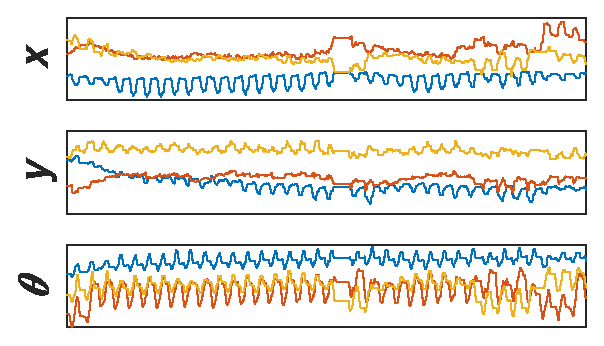
\includegraphics[width=1\textwidth]{crdDat.eps}
		\caption{Smarticle coordinates and angles as tracked from experiments \label{fig:crdDat}}
	\end{subfigure}
	\begin{subfigure}[t]{0.4\textwidth}
		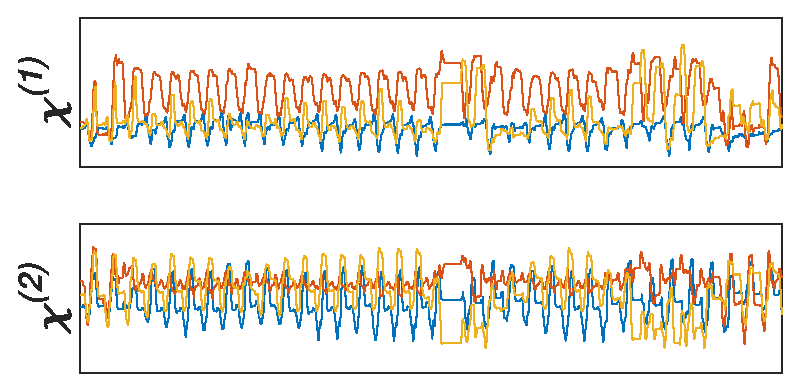
\includegraphics[width=1\textwidth]{relDat.eps}
		\caption{Rotationally invariant observables: c.o.m. coordinate as seen in the reference frame of each smarticle \label{fig:relDat}}
	\end{subfigure}
	\begin{subfigure}[t]{0.4\textwidth}
		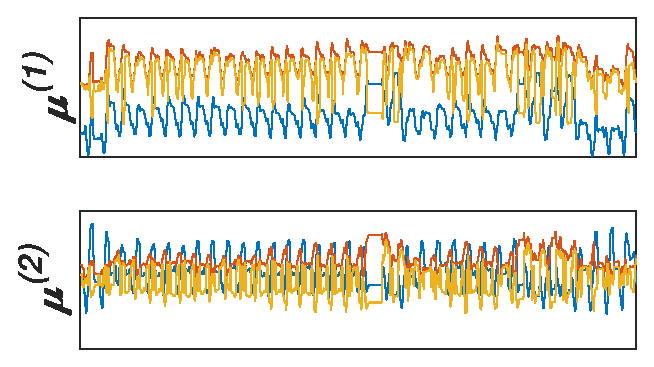
\includegraphics[width=1\textwidth]{piDat.eps}
		\caption{Permutation invariant observables: first 3 moments of the distributions in \ref{fig:relDat} \label{fig:piDat}}
	\end{subfigure}
	\begin{subfigure}[t]{0.5\textwidth}
		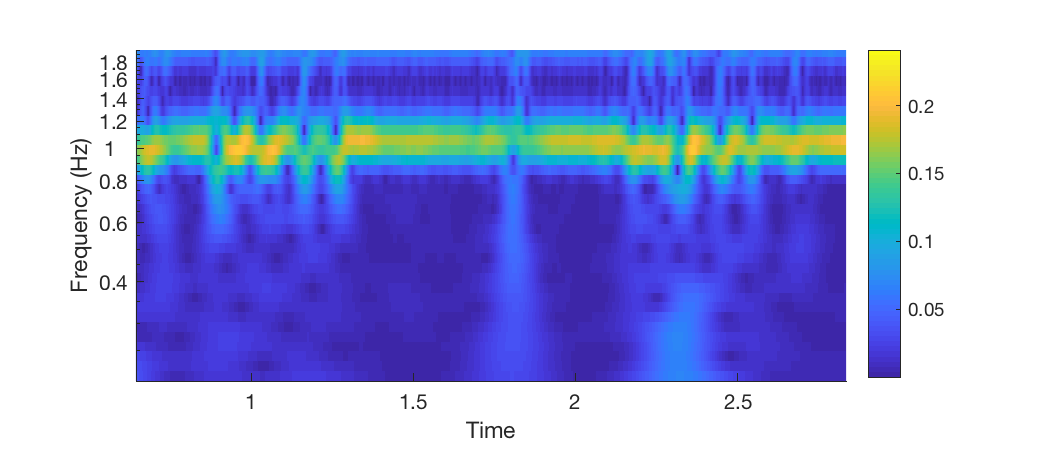
\includegraphics[width=1\textwidth]{wavelet.eps}
		\caption{Wavelet transform of one of the curves in \ref{fig:piDat}. We choose the values along the bright line for our feature vector. \label{fig:wavelet}}
	\end{subfigure}
	
	\caption{Data processing steps} \label{fig:1}
\end{figure}

\subsection{Modding out symmetries}
We begin by constructing functions of the raw data that are invariant under the symmetries we mentioned, but still sensitive to the information we may care about. The two symmetries are global rotations and permutation. To take care of the first, we find the coordinates of the c.o.m. $ \vec{X}= \frac{1}{3} \sum_i \vec{x}_i $ (note: permutation invariant) in the reference frame of each smarticle: $ \vec{\chi}_i \equiv \mathcal{R}(\theta_i) \cdot (\vec{X} - \vec{x}_i) $, where $ \mathcal{R}(\theta_i) $ is the rotation matrix for $ i $-th smarticle (fig \ref{fig:relDat}). Note that this is not a perfect choice: it is entirely invariant under c.o.m. translations (which is relevant, but we assume it to be small for a confined system), and smarticle orientation matters more the further it is from c.o.m. (so we must assume that their distance to c.o.m. stays relatively constant). We can often get away with such imperfect choices because we have so much overloaded data for the questions. 

Next, the permutation-invariant functions we choose are just the first three moments of the distribution of the three $ \{\chi_i\} $ at any fixed time. In order for these functions to have relatively similar sensitivity to changes in raw data, it helps to ensure that they have the same units -- by raising them to the appropriate fractional powers. I.e., $ \mu_1 = \frac{1}{3} \sum_i \chi_i $, $ \mu_2 = \sqrt{\frac{1}{3} \sum_i (\chi_i-\mu_1)^2} $, $ \mu_3 = \sqrt[3]{\frac{1}{3} \sum_i (\chi_i-\mu_1)^3} $ (fig. \ref{fig:piDat}). Note also that up to 3, these are the same as the cumulants -- which may be a better alternative for more smarticles.

\subsection{Capturing dynamics}
Now we can proceed to dealing with the fact that behaviors we are looking for are dynamic states, and thus depend on multiple time-points. We thus want to construct some feature vector that captures the dynamics. The simplest idea of simply stacking $ \mu_i $ at different time-points on top of each other is not obviously wrong, but will give a feature vector that is very sensitive to the noise. Instead, the dynamical features we are looking for are better captured by Fourier modes. Further, since the dynamical phase can change on the time-scale of a few arm oscillations, we don't want to transform the entire time-series, but instead consider a continuous wavelet transform of the data (fig. \ref{fig:wavelet}). This beautifully separates out behaviors on different time-scales, and we can choose our feature vector based on the time-scale(s) we most care about. The simplest choice here is to take the time-scale corresponding to one gait-period -- since most of the activity happens there. Again, this is throwing away lots of data, but since at the end we just care about some low-dimensional behavior space, we are still left with more than enough (including other time-scales had little effect). 

This way our feature vector consists of 6 complex numbers (3 moments for each dimension of the 2D $ \chi $ vector). We do care about relative phase of oscillation in the wavelet transform -- to keep this in the most unbiased way, we simply take the 36 possible differences between the 6 complex numbers, and then take their absolute value. While this makes the feature vector unnecessarily long, this is fine since we only care about the relative distances between these, and duplicate vector components will simply sum up.

\subsection{Dimensional reduction and clustering}
Now that we have our feature vector, we can dimensionally reduce or cluster the data. The former is, in a sense, a ``smoother,'' less dramatic operation, and thus turns out to produce more accurate results. We can understand this by realizing that in either case, the goal is to preserve pair-wise distances as best as possible, and this is much easier to accomplish if you allow points to be placed anywhere in the $ \mathbb{R}^2 $ plane, rather than in one of 5 discrete states. Curiously, clustering even works better when performed on dimensionally reduced, rather than original data. The other advantage of dimensionally reducing first is that this gives us more information about how the data is distributed, without imposing the assumption that it is well-clustered. 

\begin{figure}
	\begin{subfigure} [t]{0.45\textwidth}
		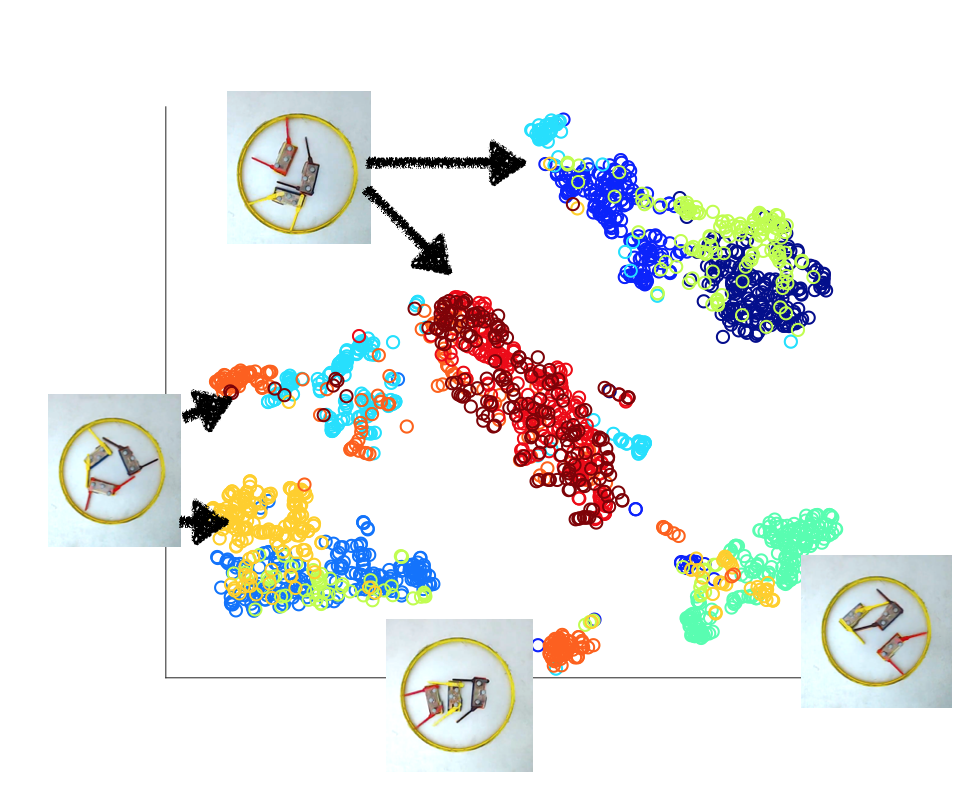
\includegraphics[width=\textwidth]{dimRedExp.png}
		\caption{Experiment \label{fig:dimRedExp}}
	\end{subfigure}
	\begin{subfigure} [t]{0.45\textwidth}
		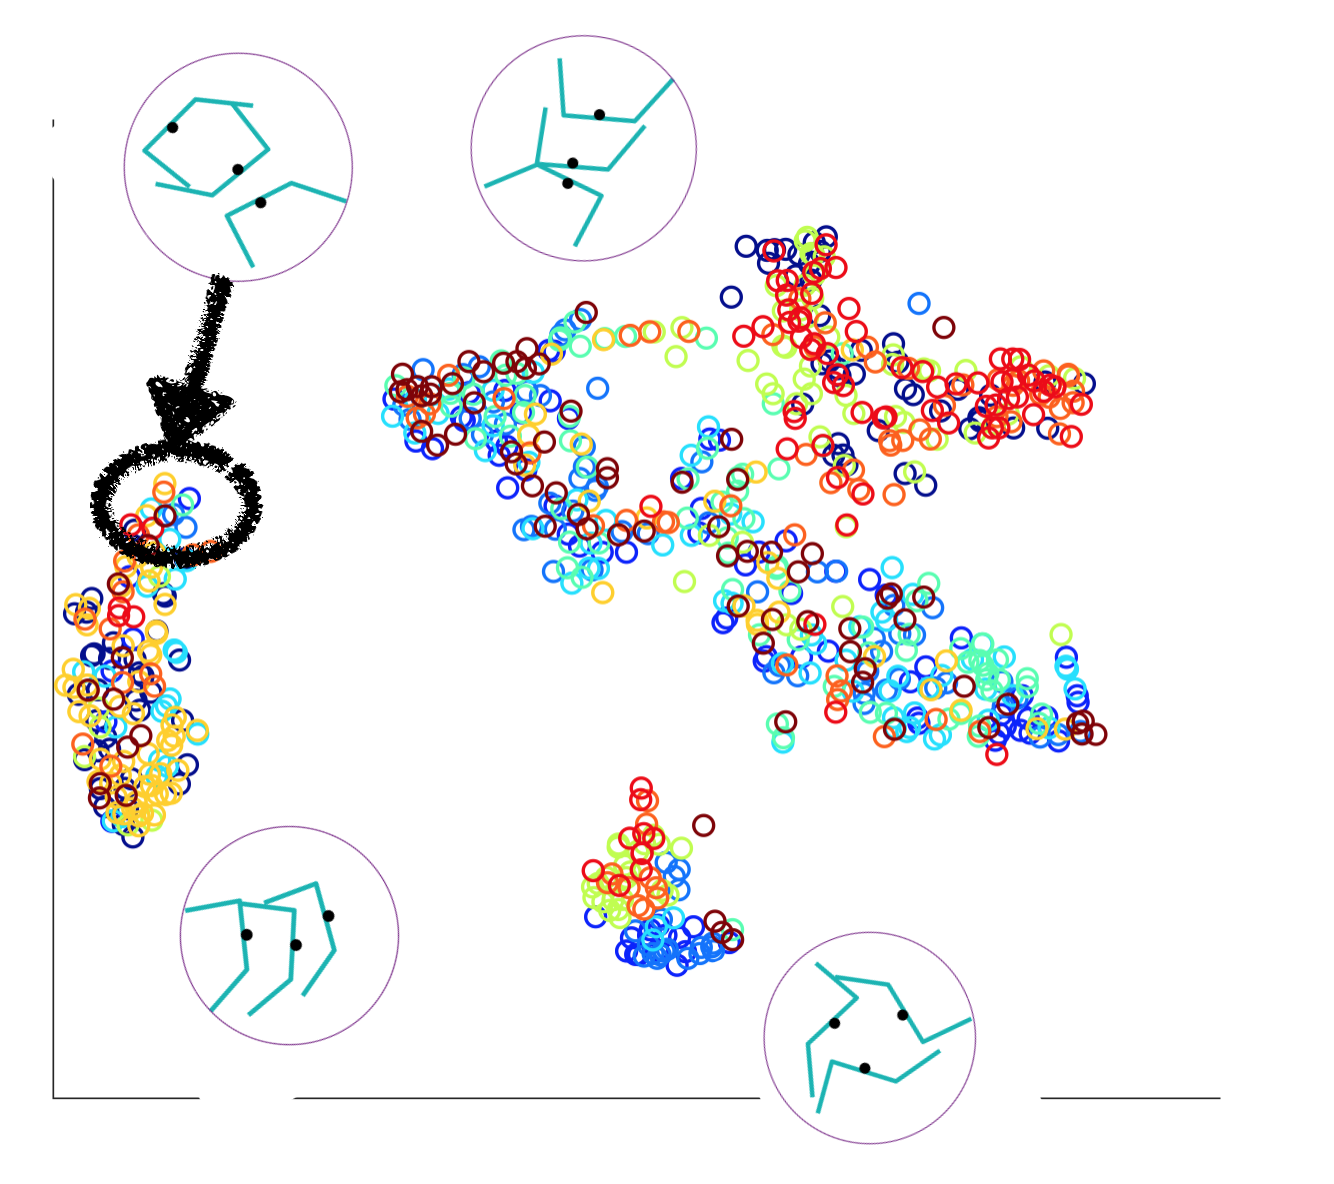
\includegraphics[width=\textwidth]{dimRedSim.png}
		\caption{Simulation \label{fig:dimRedSim}}
	\end{subfigure}
	\caption{Dimensionally reduced data. Insets show what sort of behavior each cluster corresponds to. Note that the cluster positions in the two plots are unrelated as the 2D embedding was done separately on two data sets. Color indicates different trials of the same experiment -- confirming that the behaviors are reproducible.}
\end{figure}

We use Matlab's built-in t-Distributed Stochastic Neighbor Embedding (tSNE) algorithm, which basically tries to embed the data in a 2D space preserving all the pair-wise distances as much as possible (fig. \ref{fig:dimRedExp}). It has the effect of largely preserving, or even highlighting, clusters in the original data, but also allows visualizing transitions between them and other hierarchical structure in the data. Note that the two pairs of clusters corresponding to the same pictures are chiral complements (the other two clusters correspond to non-chiral states). In section \ref{sec:dynPhaseTrans} below we will cluster this data and study the slow transition statistics between different dynamical phases.



\section{Random dynamical systems}
\subsection{Random Markov process}
\subsection{Diffusion in random medium}
\subsection{Random discrete map}
\subsection{Max-entropy modelling}

%\nocite{*}
\bibliographystyle{unsrt}
%\bibliography{../_data/14654301E131WECPZ6ZSATT3H7YHJ7G6D2E8/default_files/non-equilibSM}
\bibliography{/Users/pchvykov/Documents/GoogleDrive/MIT/RESEARCH/_data/14654301E131WECPZ6ZSATT3H7YHJ7G6D2E8/default_files/non-equilibSM.bib}

\end{document}